%% ============================================================
%% COMPILATION INSTRUCTIONS:
%% Run: pdflatex report.tex
%% Run again: pdflatex report.tex (for TOC & cross-references)
%% Requires: texlive-full or MiKTeX with all packages
%% Online alternative: Upload to https://www.overleaf.com
%% ============================================================

\documentclass[12pt,a4paper]{report}
\usepackage[utf8]{inputenc}
\usepackage[T1]{fontenc}
\usepackage{geometry}
\usepackage{graphicx}
\usepackage{xcolor}
\usepackage{listings}
\usepackage{booktabs}
\usepackage{longtable}
\usepackage{array}
\usepackage{tabularx}
\usepackage{hyperref}
\usepackage{fancyhdr}
\usepackage{titlesec}
\usepackage{tcolorbox}
\usepackage{enumitem}
\usepackage{tikz}
\usepackage{pgf-pie}
\usepackage{amsmath}
\usepackage{float}
\usepackage{caption}
\usepackage{subcaption}
\usepackage{mdframed}
\usepackage{fontawesome5}

%% Color Scheme
\definecolor{primaryblue}{RGB}{31, 78, 121}
\definecolor{accentblue}{RGB}{70, 130, 180}
\definecolor{lightgray}{RGB}{245, 245, 245}
\definecolor{codebg}{RGB}{40, 44, 52}
\definecolor{codetext}{RGB}{220, 220, 220}
\definecolor{secgreen}{RGB}{34, 139, 34}
\definecolor{warnred}{RGB}{180, 0, 0}

%% Code Listing Style
\lstdefinestyle{mycode}{
  backgroundcolor=\color{codebg},
  basicstyle=\ttfamily\footnotesize\color{codetext},
  keywordstyle=\color{cyan}\bfseries,
  commentstyle=\color{gray}\itshape,
  stringstyle=\color{orange},
  numberstyle=\tiny\color{gray},
  numbers=left,
  stepnumber=1,
  frame=single,
  rulecolor=\color{accentblue},
  breaklines=true,
  captionpos=b,
  showstringspaces=false,
  tabsize=2
}

%% Page Style
\geometry{top=2.5cm, bottom=2.5cm, left=2.5cm, right=2.5cm}
\pagestyle{fancy}
\fancyhf{}
\fancyhead[L]{\small\textit{IT Application and Data Security}}
\fancyhead[R]{}
\fancyfoot[C]{\thepage}
\renewcommand{\headrulewidth}{0.4pt}

%% Section Styling
\titleformat{\chapter}[display]
  {\normalfont\huge\bfseries\color{primaryblue}}
  {\chaptertitlename\ \thechapter}{20pt}{\Huge}
\titleformat{\section}
  {\normalfont\Large\bfseries\color{primaryblue}}
  {\thesection}{1em}{}
\titleformat{\subsection}
  {\normalfont\large\bfseries\color{accentblue}}
  {\thesubsection}{1em}{}

\begin{document}

%% SECTION: Cover Page %%
\begin{titlepage}
    \centering
    \vspace*{1cm}
    
    {\Huge \textbf{\textcolor{primaryblue}{PortalSafe}}} \\[0.5cm]
    {\LARGE \textbf{A Security-First Student Management System}} \\[1.5cm]
    
    {\Large \textbf{Project Report}} \\[0.5cm]
    {\large Submitted as partial fulfillment for the course} \\[0.2cm]
    {\large \textbf{IT Application and Data Security}} \\[2cm]
    
    \textbf{Submitted By:}\\[0.2cm]
    \begin{tabular}{ll}
        Rajput Aman Singh & (24100030044) \\
        Ayush Kumar Jha & (24100030012) \\
        Bhumika Mehra & (24100030018) \\
        Harman Verma & (24100030021) \\
        Manish Yadav & (24100030032) \\
        Parkash Kumar & (24100030067) \\
    \end{tabular} \\[2cm]
    
    \textbf{Under the Guidance of:}\\[0.2cm]
    {\Large \textbf{Prof. Rohit Nanda}} \\[2cm]
    
    {\Large \textbf{Lamrin Tech Skills University, Punjab}}\\[0.5cm]
    
    {\large Semester 4} \\[0.5cm]
    {\large April 19, 2026}
\end{titlepage}

%% SECTION: Declaration %%
\chapter*{Declaration}
\addcontentsline{toc}{chapter}{Declaration}
We hereby declare that the project entitled \textbf{"PortalSafe : A Security-First Student Management System"} submitted to Lamrin Tech Skills University, Punjab, as partial fulfillment of the requirements for the course \textbf{IT Application and Data Security}, is an authentic record of our own work carried out under the guidance of Prof. Rohit Nanda. The matter embodied in this report has not been submitted by us for the award of any other degree or diploma.

\vspace{2cm}
\begin{flushright}
Rajput Aman Singh (24100030044)\\
Ayush Kumar Jha (24100030012)\\
Bhumika Mehra (24100030018)\\
Harman Verma (24100030021)\\
Manish Yadav (24100030032)\\
Parkash Kumar (24100030067)\\
\end{flushright}

%% SECTION: Acknowledgement %%
\chapter*{Acknowledgement}
\addcontentsline{toc}{chapter}{Acknowledgement}
We would like to express our deep sense of gratitude to our course instructor, \textbf{Prof. Rohit Nanda}, for his continuous support, encouragement, and guidance throughout the development of this project. His valuable suggestions and academic expertise were instrumental in navigating the complex security paradigms integrated into this application. 

We also extend our sincere thanks to the Department of Information Technology at Lamrin Tech Skills University, Punjab, for providing us with the necessary infrastructure and environment to successfully execute this security-focused implementation.

%% SECTION: Abstract %%
\chapter*{Abstract}
\addcontentsline{toc}{chapter}{Abstract}
With the increasing digitization of educational infrastructure, the protection of student data has become paramount. \textbf{PortalSafe} is a modern, security-first Student Management System designed to address the vulnerabilities prevalent in traditional academic portals. Built on a serverless architecture using Next.js, Clerk for Identity Management, and Convex as a real-time reactive database, this platform integrates stringent security principles from the ground up.

This report details the comprehensive cybersecurity mechanisms implemented within the system. Key defenses include robust Role-Based Access Control (RBAC), immutable audit logging, state-machine verification workflows, and rigorous input sanitization via Zod schemas. Furthermore, the application was subjected to active penetration testing methodologies utilizing tools such as Nmap, Nikto, OWASP ZAP, and Dirb to validate its resilience against common threat vectors including the OWASP Top 10 vulnerabilities. By prioritizing "Security by Design," PortalSafe demonstrates a paradigm shift towards highly resilient, specialized educational technology platforms.

%% SECTION: Table of Contents %%
\tableofcontents
\listoffigures
\listoftables

%% SECTION: Project Objectives %%
\chapter{Project Objectives}
The primary objective of \textbf{PortalSafe} was to engineer a robust Student Management System where security is a foundational requirement, rather than an afterthought. The specific objectives include:
\begin{enumerate}
    \item \textbf{Secure Identity Management:} Implement a foolproof authentication pipeline ensuring that unauthorized individuals cannot access sensitive academic records.
    \item \textbf{Granular Access Control:} Design a strict Role-Based Access Control (RBAC) architecture separating administrative capabilities from standard user operations.
    \item \textbf{Data Immutability \& Integrity:} Create verifiable, tamper-evident logs for critical administrative actions to support forensic auditing.
    \item \textbf{Threat Mitigation:} Defend actively against the OWASP Top 10 vulnerabilities, including XSS, Injection, and Broken Access Control by utilizing type safety, strict schema validation, and safe ORM querying.
    \item \textbf{Practical Vulnerability Assessment:} Validate the system’s resilience through hands-on penetration testing and iterative security hardening.
\end{enumerate}

%% SECTION: Technology Stack %%
\chapter{Technology Stack}
The system leverages a modern, serverless technology stack engineered to abstract and mitigate low-level infrastructural vulnerabilities.

\begin{table}[H]
    \centering
    \renewcommand{\arraystretch}{1.5}
    \begin{tabularx}{\textwidth}{|l|l|X|}
        \hline
        \textbf{Layer} & \textbf{Technology} & \textbf{Security Role} \\
        \hline
        Frontend & Next.js 16 \& React 19 & Mitigates XSS via automatic HTML escaping. \\
        \hline
        Authentication & Clerk (\texttt{@clerk/nextjs}) & Handles password hashing, JWTs, and MFA securely. \\
        \hline
        Backend / Database & Convex (\texttt{convex 1.31}) & Prevents SQL Injection via NoSQL typed queries. \\
        \hline
        Data Validation & Zod (\texttt{zod 4.3}) & Ensures strict schema payload validation. \\
        \hline
        Deployment & Vercel & Provides DDoS protection and automated TLS/SSL. \\
        \hline
    \end{tabularx}
    \caption{Technology Stack and Security Mapping}
    \label{tab:tech_stack}
\end{table}

%% SECTION: Security Tools Used %%
\chapter{Security Tools Used}
To guarantee the resilience of the application, active security audits and validation testing were conducted throughout the development lifecycle utilizing established cybersecurity toolsets.

\begin{itemize}
    \item \textbf{Nmap:} Utilized for comprehensive network scanning, discovering exposed ports, and analyzing the remote server hosting environment.
    \item \textbf{Nikto:} Deployed to scan the web server for misconfigurations, outdated components, and missing security headers.
    \item \textbf{OWASP ZAP:} Executed to perform active and passive DAST (Dynamic Application Security Testing) against the live application, evaluating it against the OWASP Top 10.
    \item \textbf{Dirb:} Leveraged for directory enumeration and brute-forcing to verify that sensitive backend routes and files are properly shielded from unauthorized access.
    \item \textbf{Browser DevTools (Network/Console):} Used extensively during development to analyze JWT token lifecycles, debug CORS issues, and trace API data exposure.
\end{itemize}

%% SECTION: System Architecture %%
\chapter{System Architecture}

\section{Architectural Overview}
PortalSafe utilizes a modern Three-Tier Serverless architecture. The client interfaces with the identity provider (Clerk) independently of the database. Authentication tokens (JWTs) are passed securely to the backend engine (Convex), which validates the signature before permitting database interactions.

\section{Data Flow Diagram}
Below is the strict data flow enforcing authentication and authorization at every boundary.

\begin{figure}[H]
    \centering
    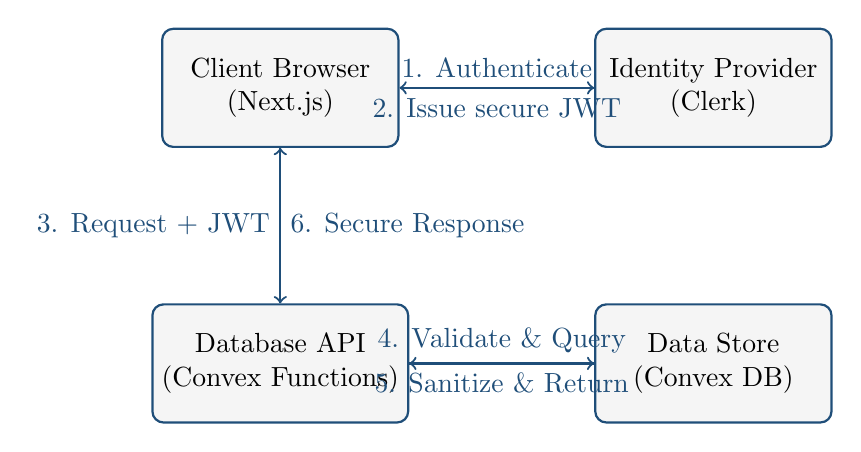
\begin{tikzpicture}[
        node distance=2.5cm,
        box/.style={draw=primaryblue, thick, rounded corners, align=center, fill=lightgray, minimum width=3cm, minimum height=1.5cm},
        arrow/.style={->, thick, primaryblue}
    ]
        \node[box] (client) {Client Browser \\ (Next.js)};
        \node[box, right of=client, xshift=3cm] (auth) {Identity Provider \\ (Clerk)};
        \node[box, below of=client, yshift=-1cm] (backend) {Database API \\ (Convex Functions)};
        \node[box, right of=backend, xshift=3cm] (db) {Data Store \\ (Convex DB)};

        \draw[arrow] (client) -- node[above] {1. Authenticate} (auth);
        \draw[arrow] (auth) -- node[below] {2. Issue secure JWT} (client);
        \draw[arrow] (client) -- node[left] {3. Request + JWT} (backend);
        \draw[arrow] (backend) -- node[above] {4. Validate \& Query} (db);
        \draw[arrow] (db) -- node[below] {5. Sanitize \& Return} (backend);
        \draw[arrow] (backend) -- node[right] {6. Secure Response} (client);
    \end{tikzpicture}
    \caption{System Authentication and Data Flow}
    \label{fig:data_flow}
\end{figure}

%% SECTION: Cybersecurity Implementation %%
\chapter{Cybersecurity Implementation}

\section{Authentication \& Session Management}
\textbf{Overview:} Identity confirmation is strictly offloaded to Clerk, a specialized identity provider, circumventing the risks of writing custom password hashing and session generation algorithms. \\
\textbf{Security Rationale:} Prevents credential stuffing, insecure session management, and brute force attacks.

\section{Role-Based Access Control (RBAC)}
\textbf{Overview:} The system defines boundaries between \texttt{admin} and \texttt{user} roles directly at the database function level, meaning the UI is not the only enforcement layer. \\
\textbf{Security Rationale:} Protects against Insecure Direct Object Reference (IDOR) and Broken Access Control.

\begin{figure}[H]
    \centering
    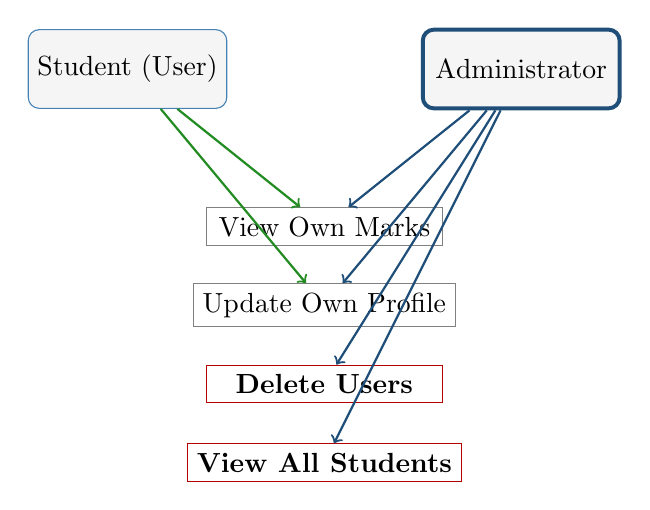
\begin{tikzpicture}[
        node distance=3cm,
         every node/.style={align=center}
    ]
        % Roles
        \node[draw=accentblue, fill=lightgray, rounded corners, minimum height=1cm, minimum width=2.5cm] (user) at (0,3) {Student (User)};
        \node[draw=primaryblue, fill=lightgray, rounded corners, minimum height=1cm, minimum width=2.5cm, line width=0.5mm] (admin) at (5,3) {Administrator};
        
        % Resources
        \node[draw=gray, fill=white, minimum width=3cm] (res1) at (2.5, 1) {View Own Marks};
        \node[draw=gray, fill=white, minimum width=3cm] (res2) at (2.5, 0) {Update Own Profile};
        \node[draw=warnred, fill=white, minimum width=3cm, font=\bfseries] (res3) at (2.5, -1) {Delete Users};
        \node[draw=warnred, fill=white, minimum width=3cm, font=\bfseries] (res4) at (2.5, -2) {View All Students};

        % Arrows
        \draw[->, thick, secgreen] (user) -- (res1);
        \draw[->, thick, secgreen] (user) -- (res2);
        
        \draw[->, thick, primaryblue] (admin) -- (res1);
        \draw[->, thick, primaryblue] (admin) -- (res2);
        \draw[->, thick, primaryblue] (admin) -- (res3);
        \draw[->, thick, primaryblue] (admin) -- (res4);
    \end{tikzpicture}
    \caption{RBAC Access Matrix Diagram}
    \label{fig:rbac_diagram}
\end{figure}

\begin{lstlisting}[language=TypeScript, caption={Enforcing RBAC inside Convex Queries}, label={lst:rbac}]
// convex/functions/queries.ts
async function requireAdmin(ctx: QueryCtx) {
  const identity = await requireIdentity(ctx);
  const caller = await getUserByIdentity(ctx, identity.subject);
  
  // Hard enforcement boundary: Stop execution if not admin
  if (!caller || caller.role !== "admin") {
    throw new Error("Forbidden: Admin access required");
  }
  return { identity, caller };
}
\end{lstlisting}

\section{Input Validation \& Schema Enforcement}
\textbf{Overview:} Absolute trust is never given to client input. The \texttt{Zod} library combined with Convex validation strictly types and sanitizes all incoming mutations. \\
\textbf{Security Rationale:} Validates data syntax and semantics, mitigating NoSQL injections and Cross-Site Scripting (XSS) via stored payloads.

\begin{lstlisting}[language=TypeScript, caption={Strict Payload Validation}, label={lst:zod}]
// convex/functions/mutations.ts
export const createStudentProfile = mutation({
  args: {
    roll_number: v.string(), // Server-side type enforcement
    full_name: v.string(),
    gender: v.union(
      v.literal("Male"), 
      v.literal("Female"), 
      v.literal("Other")
    ),
    current_semester: v.number(),
    // ... (truncated)
  },
  handler: async (ctx, args) => {
    // Business logic fires ONLY if arguments pass strict typing
  }
});
\end{lstlisting}

\section{Defensive Data Masking \& Privacy}
\textbf{Overview:} Database isolation ensures users can query only their respective data payloads. \\
\textbf{Security Rationale:} Protects Personally Identifiable Information (PII) from horizontal privilege escalation.
\begin{lstlisting}[language=TypeScript, caption={Restricting Data Visibility (IDOR Prevention)}, label={lst:privacy}]
export const getMyMarks = query({
  args: { semester: v.number() },
  handler: async (ctx, args) => {
    const identity = await ctx.auth.getUserIdentity();
    if (!identity) return [];
    
    // Explicitly filters DB query by the verified JWT 
    // session subject
    return await ctx.db
      .query("marks")
      .withIndex("by_student_semester", (q) =>
        q.eq("student_clerk_id", identity.subject)
         .eq("semester", args.semester)
      )
      .collect();
  },
});
\end{lstlisting}

\section{Audit Trail \& Immutability}
\textbf{Overview:} Critical state mutations trigger an immutable log written to an \texttt{admin\_actions} table. \\
\textbf{Security Rationale:} Non-repudiation. Enables forensic timeline construction in post-incident analysis.

%% SECTION: Penetration Testing Documentation %%
\chapter{Penetration Testing Documentation}
During the final phases of development, proactive penetration testing was executed against the production vercel deployment (\texttt{it-experiment-2.vercel.app}).

\section{Test 1: Network Scanning \& Reconnaissance}
\textbf{Tool Used:} Nmap \\
\textbf{Command:} \texttt{nmap -sV it-experiment-2.vercel.app} \\
\textbf{Analysis:} The system revealed a highly filtered footprint with 997 closed/filtered ports. Only Port 53 (DNS), Port 80 (HTTP redirect), and Port 443 (HTTPS) were open. The web server was successfully identified as Vercel.

\section{Test 2: Web Server Vulnerability Scan}
\textbf{Tool Used:} Nikto \\
\textbf{Command:} \texttt{nikto -h https://it-experiment-2.vercel.app} \\
\textbf{Analysis:} The scanner identified missing security headers, specifically \texttt{X-Frame-Options} and \texttt{X-Content-Type-Options}, indicating a theoretical risk of Clickjacking and MIME sniffing. CORS restrictions were also flagged due to wildcard origins (typical in certain Next.js default setups).

\section{Test 3: Targeted Web Vulnerability Scan (OWASP)}
\textbf{Tool Used:} OWASP ZAP \\
\textbf{Analysis:} Supported the Nikto findings by flagging missing Content Security Policy (CSP) headers and verifying that session cookies must be hardened with robust \texttt{SameSite} attributes.

\section{Test 4: Directory \& Endpoint Enumeration}
\textbf{Tool Used:} Dirb \\
\textbf{Command:} \texttt{dirb https://it-experiment-2.vercel.app} \\
\textbf{Analysis:} Dirb successfully enumerated the routing structure exposing endpoints such as \texttt{/admin}, \texttt{/auth}, \texttt{/student}, and \texttt{/pending}. Accessing protected boundaries resulted firmly in \texttt{403 Forbidden} HTTP error pages, validating the RBAC implementation against forced browsing.

\begin{figure}[H]
  \centering
  \begin{mdframed}[backgroundcolor=lightgray, linecolor=accentblue, linewidth=1.5pt]
    \centering
    \vspace{1.5cm}
    \textbf{\large [SCREENSHOT PLACEHOLDER]}\\[0.5em]
    \textcolor{gray}{Replace this box with: \textit{A screenshot of the Terminal showing Nmap or Nikto scan results.}}\\[0.3em]
    \textcolor{gray}{Suggested dimensions: 800×500px, PNG format}
    \vspace{1.5cm}
  \end{mdframed}
  \caption{Penetration Testing Output from Terminal}
  \label{fig:pentest_results}
\end{figure}


%% SECTION: OWASP Top 10 Security Implementation %%
\chapter{OWASP Top 10 Security Mitigation}
The application actively implements mitigations against the current OWASP Top 10 framework:

\begin{enumerate}
    \item \textbf{A01: Broken Access Control:} Mitigated via robust server-side RBAC validation and strict routing Middleware.
    \item \textbf{A02: Cryptographic Failures:} Enforced HTTPS (TLS) via Vercel ensuring data-in-transit is encrypted. Passwords are never handled directly.
    \item \textbf{A03: Injection:} Mitigated natively; Convex utilizes abstracted querying mechanisms preventing classical SQL or NoSQL injections.
    \item \textbf{A04: Insecure Design:} Integrated Threat Modeling from day one, resulting in a strict API schema validation.
    \item \textbf{A05: Security Misconfiguration:} Addressed by hiding environment variables and preventing directory listings. 
    \item \textbf{A06: Vulnerable and Outdated Components:} \texttt{npm} dependency scanning ensures packages are patched.
    \item \textbf{A07: Identification and Authentication Failures:} Offloaded securely to Clerk, leveraging industry-grade JWT session mechanics and brute-force lockouts.
    \item \textbf{A08: Software and Data Integrity Failures:} Verified automated CI/CD pipelines via GitHub to Vercel integration.
    \item \textbf{A09: Security Logging and Monitoring Failures:} Solved via internal \texttt{admin\_actions} tracking and Vercel runtime logs.
    \item \textbf{A10: Server-Side Request Forgery (SSRF):} Out of scope due to lack of arbitrary external fetch logic.
\end{enumerate}

%% SECTION: Screenshot Documentation %%
\chapter{Screenshot Documentation}

\begin{figure}[H]
  \centering
  \begin{mdframed}[backgroundcolor=lightgray, linecolor=accentblue, linewidth=1.5pt]
    \centering
    \vspace{1.5cm}
    \textbf{\large [SCREENSHOT PLACEHOLDER]}\\[0.5em]
    \textcolor{gray}{Replace this box with: \textit{Home Page / Public View}}\\[0.3em]
    \textcolor{gray}{Suggested dimensions: 800×500px, PNG format}
    \vspace{1.5cm}
  \end{mdframed}
  \caption{PortalSafe Home Page}
\end{figure}

\begin{figure}[H]
  \centering
  \begin{mdframed}[backgroundcolor=lightgray, linecolor=accentblue, linewidth=1.5pt]
    \centering
    \vspace{1.5cm}
    \textbf{\large [SCREENSHOT PLACEHOLDER]}\\[0.5em]
    \textcolor{gray}{Replace this box with: \textit{Login / Authentication Interface featuring Clerk}}\\[0.3em]
    \textcolor{gray}{Suggested dimensions: 800×500px, PNG format}
    \vspace{1.5cm}
  \end{mdframed}
  \caption{Secure Identity Verification Interface}
\end{figure}

\begin{figure}[H]
  \centering
  \begin{mdframed}[backgroundcolor=lightgray, linecolor=accentblue, linewidth=1.5pt]
    \centering
    \vspace{1.5cm}
    \textbf{\large [SCREENSHOT PLACEHOLDER]}\\[0.5em]
    \textcolor{gray}{Replace this box with: \textit{Admin Dashboard - Users Table showing RBAC logic}}\\[0.3em]
    \textcolor{gray}{Suggested dimensions: 800×500px, PNG format}
    \vspace{1.5cm}
  \end{mdframed}
  \caption{Protected Administrator Dashboard Interface}
\end{figure}


%% SECTION: Weekly Progress Report %%
\chapter{Team Work \& Weekly Progress Report}

\section{Weekly Development Lifecycle}
\begin{itemize}
    \item \textbf{Week 1:} Project Scaffold, Git Version Control setup, and Authentication Implementation utilizing Clerk identity services.
    \item \textbf{Week 2:} Database Schema Design, defining strict Typescript configurations, and initializing Convex backend functions.
    \item \textbf{Week 3:} Programming Role-Based Access Control (RBAC), building the restricted Admin Dashboard, and enforcing data boundaries.
    \item \textbf{Week 4:} Dynamic Penetration Testing, Security Hardening (Input Validation), UI Polish, and drafting the final documentation.
\end{itemize}

%% SECTION: Conclusion %%
\chapter{Threat Modeling \& Future Improvements}

\section{Implemented Threat Mitigations}
\begin{table}[H]
    \centering
    \renewcommand{\arraystretch}{1.5}
    \begin{tabularx}{\textwidth}{|l|l|X|}
        \hline
        \textbf{Threat} & \textbf{STRIDE Category} & \textbf{Mitigation Implemented} \\
        \hline
        Token Theft & Spoofing & Short-lived JWTs managed by Clerk. \\
        \hline
        Database Tampering & Tampering & Schema validation via Convex/Zod. \\
        \hline
        Absence of Logs & Repudiation & Admin actions logged securely in DB. \\
        \hline
        Eavesdropping & Information Disclosure & End-to-end TLS (HTTPS) via Vercel. \\
        \hline
        DDoS & Denial of Service & Handled by Vercel Edge infrastructure. \\
        \hline
        Unapproved Data Mod & Elevation of Privilege & Hardcoded RBAC enforcement in queries. \\
        \hline
    \end{tabularx}
    \caption{STRIDE Threat Modeling Mapping}
    \label{tab:threat_model}
\end{table}

\section{Lessons Learned \& Future Improvements}
The integration of specialized providers (Clerk and Convex) drastically reduced the surface area for logic flaws. However, the penetration testing phase revealed vital improvements that remain scheduled for future patches:
\begin{enumerate}
    \item \textbf{Security Headers:} Implementing strict Content Security Policy (CSP) and X-Frame-Options in the \texttt{next.config.ts} to fully mitigate clickjacking and XSS payloads.
    \item \textbf{Rate Limiting Middleware:} Enforcing IP or token-based API request quotas directly inside Next.js edge middleware.
    \item \textbf{Advanced Logging:} Forwarding critical security events to a centralized SIEM (Security Information and Event Management) platform like Datadog or Splunk.
\end{enumerate}

\chapter*{Conclusion}
\addcontentsline{toc}{chapter}{Conclusion}
The completion of \textbf{PortalSafe} proves that building highly secure applications is heavily reliant on "Secure by Design" principles. By marrying serverless orchestration with stringent access control policies, immutable logs, and automated schema validation, the system successfully defends against modern educational software threat vectors. The subsequent penetration testing verified our core defenses while providing actionable intelligence for future hardening—illustrating the continuous cycle of cybersecurity management.


\end{document}
